\section{Desenvolvimento}

\subsection{Desenvolvimento tecnológico como um indicador de problemas sociais}

O primeiro ponto a ser evidenciado há de ser o alicerce do argumento principal da discussão proposta: existe, de fato,
uma correlação observável entre o grau de adoção tecnológica no contexto da existência uma comunidade e a incidência de
problemas sociais --- sejam estes individuais ou sistêmicos? A verdade é que, para este tipo de questionamento, as
respostas encontradas dificilmente são achados concretos; é possível, no entanto, inferir à partir estudos estatísticos, se
há, ou não há, base para discussão acadêmica sobre dado postulado. No caso em questão, como pode-se intuir puramente à partir
da quantidade de estudos e ensaios publicados tratando do tema nas últimas décadas
\cite{secretariat1977,marien1977415}, sugerir que o progresso tecnológico da sociedade pode
ser um fator que mantém uma correlação com tendências problemáticas no desenvolvimento e vivência dos indivíduos que a compõe
não é algo de novo e, segundo as estatísticas indicam, não é nenhum equívoco: estudos conduzidos nos últimos cinco anos
identificam que muitas características da vida moderna --- produtos da revolução industrial \textit{especialmente} acentuados na
vivência urbana --- como disparidades sociais, poluição ambiental ou escassez de \textit{greenspace} podem ser
identificados como fatores contribuintes para os níveis elevados de incidência de problemas de saúde mental observados
em populações urbanas em países desenvolvidos \cite[1]{XU2023299}.

\begin{figure}[h]
    \centering
    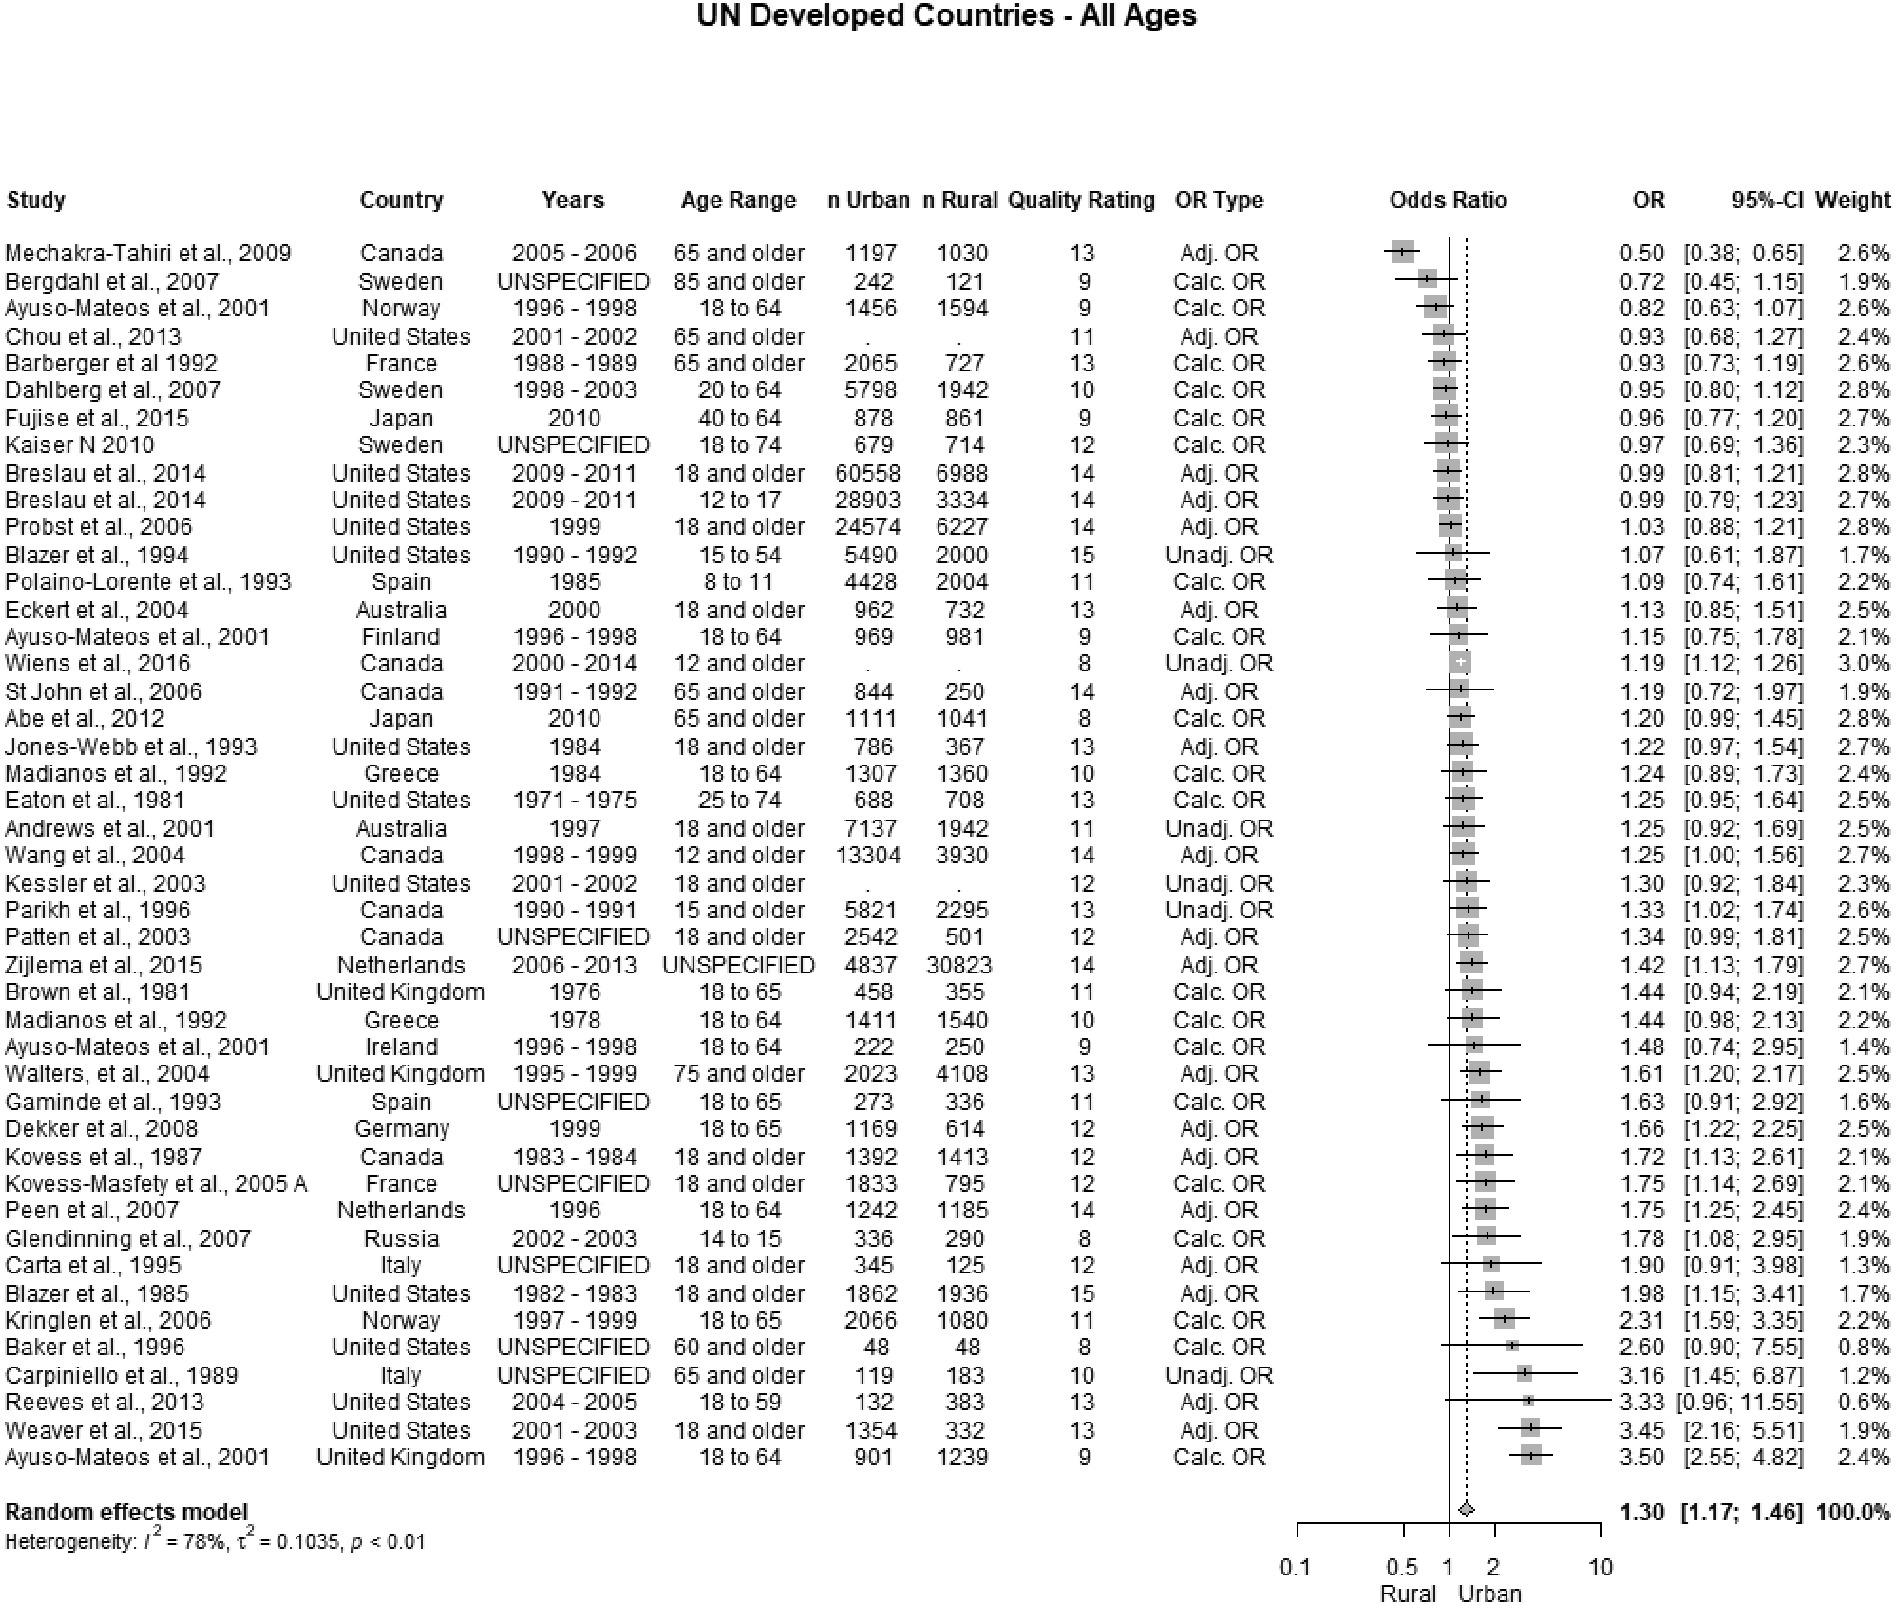
\includegraphics[width=15cm]{Content/Images/depression_rate.jpg}
    \caption{Incidência de depressão entre populações urbanas vs.\ rurais em países industrialmente desenvolvidos. Modelo
  matemático. \cite{XU2023299}}
\end{figure}

Como pode ser encontrado em estudos de até quatro décadas atrás, o grau de adoção e \gls{dependencia} de uma comunidade tem
um efeito não somente sobre a dinâmica econômica e social da realidade dos indivíduos nesta inseridos, mas pode mesmo
influenciar o condicionamento psicológico e valores característicos na paisagem cultural comunal \cite[27-30]{secretariat1977}.
Desta forma, fica evidente que os impactos da \gls{dependencia} devem ser estudados não apenas na escala \textit{macro},
mas que uma análise de escopo individual também é necessária.

\subsection{Autonomia}

A complicação atrelada de forma mais aguda a um crescente nível de \gls{dependencia} é, por definição, a perda de autonomia do
sujeito, seja ele individual ou coletivo, perante ao fim para qual a tecnologia adotada é um meio (se qualquer; como
será explorado adiante, um fator oriundo do processo pelo qual a dependência se forma é o surgimento de necessidades
artificiais à serem supridas \cite[\S59-65]{kaczynski1995}; ver parágrafo \ref{necessidades_artificiais}) e o surgimento
da relação de dependência assimétrica onde este sujeito torna-se subjugado ao provedor da tecnologia organizacional
\cite[27-30]{secretariat1977}.

A ocorrência desta espécie de relação desequilibrada segue um padrão frequentemente identificado: o processo de submissão
econômica e tecnológica é, em determinado aspecto, um processo histórico. Análise macroscópica de relações
internacionais envolvendo troca de \textit{commodities} entre nações em desenvolvimento e potências industriais reflete
este padrão de assimetria nos tipos de bens capitais trocados por cada parte, que se manifesta na escala individual
através da (escassez de) diversidade de oportunidades econômicas disponíveis para indivíduos e comunidades que compõem
sociedades tecnologicamente subdesenvolvidas como consequência da desvantagem sistêmica manifestada pela diferença no
grau de desenvolvimento tecnológico e, assim, nos meios de produção \cite[27-30]{secretariat1977}. Desta forma, ao
analisarmos esta situação sob o escopo da experiência individual, observamos a emergência de um outro padrão cujo o
estudo é instrumental para a compreensão dos impactos sociais causados pela aceleração tecnológica: a limitação da gama
de possibilidades que compõe a realidade do indivíduo como consequência da busca pelo avanço tecnológico absoluto
\cite[\S51]{kaczynski1995}.

Este padrão ocorre não apenas na variedade de atividades econômicas acessíveis para dada parcela da população, mas de
forma universal ao passo que o progresso tecnológico em si passa a significar a aceleração do próprio sistema e não mais
a priorização do avanço e melhoria da situação humana. Observa-se que o progresso tecnológico que, em um primeiro
momento, tem o propósito de possibilitar a expansão do potencial humano, logo torna-se o objeto do esforço que restringe
as liberdades do indivíduo \cite[\S127]{kaczynski1995}; como um exemplo prático, pode ser empregada uma análise do caso
do transporte motorizado, que no momento de sua invenção, apresentava uma solução para o transporte rápido entre pontos
excepcionalmente distantes --- um século após a popularização do automóvel, este tornou-se essencialmente indispensável
para a vivência moderna, como agora as cidades e os espaços de vivência são projetados para os carros, não para os
homens. Desta forma, a sociedade adequa-se para acomodar o avanço tecnológico e é moldada por ele; para
o indivíduo, o progresso inabalado da tecnologia é algo que é imposto sobre ele, sobre o qual não tem autonomia e deve,
assim como a sociedade em que está inserido, adequar-se. Quando a tecnologia em questão é de ordem organizacional (ver
glossário \cite[\S207-212]{kaczynski1995}) existe um efeito composto caracterizado por não somente a dependência sobre o
recurso em si, mas também sobre a relação com o elemento que provê esta tecnologia, que então exerce uma relação de
dominância sobre o usuário subjugado, neste caso, o indivíduo.

\subsubsection{Autonomia e independência na era digital}

\subsection{Liberdade}

\subsubsection{Necessidades artificiais}\label{necessidades_artificiais}
[\dots] O processo pelo qual as práticas de publicidade e propaganda criam necessidades que não existiam anteriormente
\cite[3]{jameshulbert1968}. No decorrer das últimas duas décadas, especialmente

